\subsubsection{User}

\vfill

\begin{figure}[H]
  \centering
  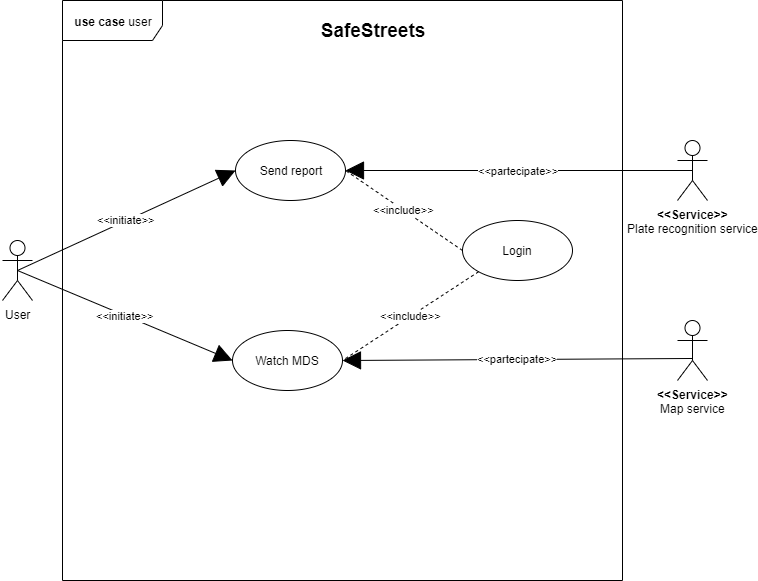
\includegraphics[width=\textwidth]{UML_diagrams/ucd_user.png}
  \caption{User use case diagram}
  \label{fig:user_ucd}
\end{figure}

\vfill
\newpage
\null


\subsubsection{Authorities}
In Fig \ref{fig:authority_ucd}, the Authority Login use case displayed in the following diagram is not related to any use case enlisted in section \ref{use_cases}. That is because the Login use case for the authority is basically the same as the user's one, indeed the only thing that changes is that the actor performs the login on the Web application instead of the mobile application.

\vfill


\begin{figure}[H]
  \centering
  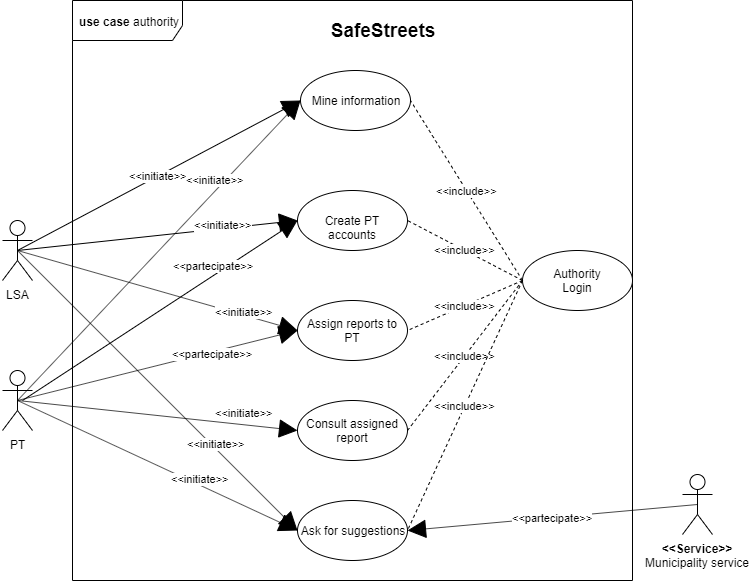
\includegraphics[width=\textwidth]{UML_diagrams/ucd_authority.png}
  \caption{Authority use case diagram}
  \label{fig:authority_ucd}
\end{figure}

\vfill
\newpage

